\documentclass[convert = false, tikz]{standalone}
\usepackage[utf8]{inputenc}
\usepackage{tikz}
\usepackage{xcolor}
\usetikzlibrary{automata, positioning, arrows}
 
% \usepackage{../../../../style_automata}

% arara: pdflatex
% arara: latexmk: { clean: partial }
\begin{document}
    \tikzset{
    node distance=1mm, % specifies the minimum distance between two nodes.
    every node/.style={draw, rectangle, minimum width=4cm, text width=3.8cm, font=\itshape, align=left, inner sep=2pt}
    }
    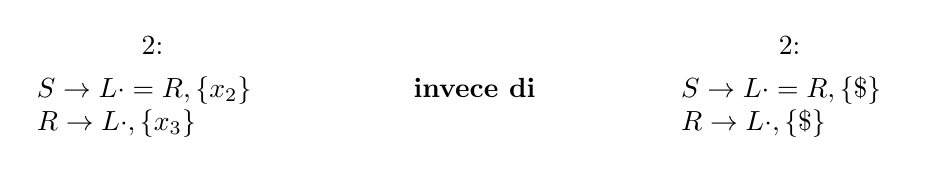
\begin{tikzpicture}[]
        % Left side
        \node [] (0) {
            \begin{tabular}{@{}l}
                $S \rightarrow L \cdot = R, \{x_2\}$ \\
                $R \rightarrow L \cdot, \{ x_3\}$ \\
            \end{tabular}
        };
        \node [above, draw=none, font=\normalfont] at (0.north) {2:}; %label
        
        % Right side
        \node [right = 5cm of 0] (1) {
            \begin{tabular}{@{}l}
                $S \rightarrow L \cdot = R, \{\$\}$ \\
                $R \rightarrow L \cdot, \{\$\}$ \\
            \end{tabular}
        };
        \node [above, draw=none, font=\normalfont] at (1.north) {2:}; %label

        % Text between nodes 1 and 3
        \path (0.east) edge [draw=none] node[pos=0.5, above, font=\bfseries, draw=none, align=center] {invece di} (1.west);
    \end{tikzpicture}
\end{document}